% !TEX TS-program = pdflatex
% !TEX encoding = UTF-8 Unicode

% This is a simple template for a LaTeX document using the "article" class.
% See "book", "report", "letter" for other types of document.

\documentclass[20pt]{article} % use larger type; default would be 10pt

\usepackage[utf8]{inputenc} % set input encoding (not needed with XeLaTeX)

%%% Examples of Article customizations
% These packages are optional, depending whether you want the features they provide.
% See the LaTeX Companion or other references for full information.

%%% PAGE DIMENSIONS
\usepackage{geometry} % to change the page dimensions
\geometry{a4paper} % or letterpaper (US) or a5paper or....
% \geometry{margin=2in} % for example, change the margins to 2 inches all round
% \geometry{landscape} % set up the page for landscape
%   read geometry.pdf for detailed page layout information

\usepackage{graphicx} % support the \includegraphics command and options

% \usepackage[parfill]{parskip} % Activate to begin paragraphs with an empty line rather than an indent

%%% PACKAGES
\usepackage{booktabs} % for much better looking tables
\usepackage{array} % for better arrays (eg matrices) in maths
\usepackage{paralist} % very flexible & customisable lists (eg. enumerate/itemize, etc.)
\usepackage{verbatim} % adds environment for commenting out blocks of text & for better verbatim
%\usepackage{subfig} % make it possible to include more than one captioned figure/table in a single float
\usepackage{mathtools}
\usepackage{graphicx} % supports images in latex
% These packages are all incorporated in the memoir class to one degree or another...

\usepackage{graphicx}
\usepackage{subcaption}

%%% Other stuff
\DeclarePairedDelimiter\ceil{\lceil}{\rceil}
\DeclarePairedDelimiter\floor{\lfloor}{\rfloor}

%%% HEADERS & FOOTERS
\usepackage{fancyhdr} % This should be set AFTER setting up the page geometry
\pagestyle{fancy} % options: empty , plain , fancy
\renewcommand{\headrulewidth}{0pt} % customise the layout...
\lhead{}\chead{}\rhead{}
\lfoot{}\cfoot{\thepage}\rfoot{}

%%% SECTION TITLE APPEARANCE
\usepackage{sectsty}
\allsectionsfont{\sffamily\mdseries\upshape} % (See the fntguide.pdf for font help)
% (This matches ConTeXt defaults)

%%% ToC (table of contents) APPEARANCE
\usepackage[nottoc,notlof,notlot]{tocbibind} % Put the bibliography in the ToC
\usepackage[titles,subfigure]{tocloft} % Alter the style of the Table of Contents
\renewcommand{\cftsecfont}{\rmfamily\mdseries\upshape}
\renewcommand{\cftsecpagefont}{\rmfamily\mdseries\upshape} % No bold!

%%% graphics path
\graphicspath{{./HW5}}

%%% END Article customizations

%%% nice things to keep around

% \noindent\rule{2cm}{0.4pt} 
%%% puts a small horizontal line

% \mathcal{O} 
%%% big O notation

%%% The "real" document content comes below...

\title{Algorithms Homework 4}
\author{Liam Dillingham}
%\date{} % Activate to display a given date or no date (if empty),
         % otherwise the current date is printed 

\begin{document}
\maketitle

\section{Question 15.2-2} 
Give a recursive algorithm MATRIX-CHAIN-MULTIPLY($A$, $s$, $i$, $j$) that actually performs the optimal matrix-chain multiplication, given the sequence of matrices $\langle A_1, A_2, ..., A_n \rangle$, the $s$ table computed  by MATRIX-CHAIN-ORDER, and the indices, $i$ and $j$. (The initial call would be MATRIX-CHAIN-MULTIPLY($A$, $s$, $1$, $n$). ). \\
\noindent\rule{2cm}{0.4pt} \\

The initial call MATRIX-CHAIN-MULTIPLY($A$, $s$, $1$, $n$) is because the initial problem is parenthesizing the initial problem: the entire list of matrices.  Then, we can start working on the subproblem(s).  The first thing to handle would be the base case.  In matrix-chain-multiply, we parenthesize, or group, matrices per the indices.  So for two indices, $i$ and $j$, we multiply, from left to right, All matrices with indices $\geq i$ up to and including all matrices with indices $\leq j$.\\ 

It should be noted that $s[i, j]$ contains a value which specifies the upper limit of parenthesization.  So the call to the algorithm should look like this: \\

MATRIX-CHAIN-MULTIPLY($A$, $s$, $i$, $s[i, j]$); \\

Where $i$ is initially $1$, and $s[i,j]$ is $s[1,n]$, which will give us the parenthesization for the entire list of matrices.  Then we will want to call MATRIX-CHAIN-MULTIPLY($A$, $s$, $i$, $s[i, j]$) again on the left and right of the parenthesization "split" to see what an optimal parenthesization is on each subproblem.  So we call the function again on the left and right intervals, and multiply their product like so: \\ 

MATRIX-CHAIN-MULTIPLY($A$, $s$, $i$, $s[i, j]$) $*$ MATRIX-CHAIN-MULTIPLY($A$, $s$, $s[i, j]+1$, $j$) \\

We should also be aware that the cost of multiplying a matrix by itself is $0$. Or rather, we do not multiply a matrix by itself. In the case where $i == j$, or that the left bounding parenthesization equals the right, we simply return the matrix at that index. Therefore, the pseudocode looks as follows:

\begin{verbatim}
MATRIX-CHAIN-MULTIPLY(A, s, i, j)
   if i == j
      return A[i] // A is an array of matrices
   return MATRIX-CHAIN-MULTIPLY(A, s, i, s[i, j]) * MATRIX-CHAIN-MULTIPLY(A, s, s[i, j] + 1, j)
\end{verbatim}

\newpage
\section{Question 15.4-2} 
Give pseudocode to reconstruct an LCS from the completed $c$ table and the original sequences $X = \langle x_1, x_2, ..., x_m \rangle$ and $Y = \langle y_1, y_2, ..., y_n \rangle$ in $\mathcal{O}(m + n)$ time, without using the $b$ table. \\ 
\noindent\rule{2cm}{0.4pt} \\

A completed C-table can be seen below:

\begin{figure}[!htbp]
  	\centering
   	\begin{subfigure}[p]{0.4\linewidth}
    	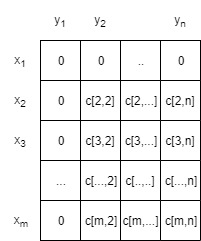
\includegraphics[width=\linewidth]{ctable.jpg}
     	\caption{Completed C-table}
   	\end{subfigure}
\end{figure} 

Where each cell corresponds to the current LCS at that point in each string. That is, at $c[3,2]$, suppose the value is $2$. That means that as of the 3rd character in $X$ and the 2nd character in $Y$, we have a subsequence of length $2$.  Thus, when we are at $c[m,n]$, we have walked the entire length of both strings.  While there are base cases where one strings and the other doesn't, this is the actual terminal state for the entire algorithm. Thus, when we reach $c[m,n]$, we can walk backwards towards $c[0,0]$ to compute the reversed LCS, and then reverse that to obtain the LCS.  The pseudocode for this can be shown below:

\newpage
\begin{verbatim}
CONSTRUCT-LCS(x, y, c)
   output = "" // Let output be an empty string to push onto
   m = x.length // length of string x
   n = y.length // length of string y

   i = m
   j = n
   for k = m + n to 1
      max = c[i - 1, j - 1]
      if c[i - 1, j] > max
         max = c[i - 1, j]
         i = i - 1
         output.push(x[i - 1])
      elseif c[i, j - 1] > max
         max = c[i, j - 1]
         j = j - 1
         output.push(y[j - 1])
      else
         i = i - 1
         j = j - 1
         output.push(x[i - 1])
   
   output.reverse()
   return output
\end{verbatim}

the loop runs $m + n$ times. and since the length of the LCS is either $m$ or $n$ then reversing the string either takes $m$ or $n$ times. Then, the runtime is either $\mathcal{O}(2m + n)$ or $\mathcal{O}(m + 2n)$ which, asymptotically is $\mathcal{O}(m + n)$.

\end{document}
